%% OfficeFloor - http://www.officefloor.net
%% Copyright (C) 2013 Daniel Sagenschneider
%%
%% This program is free software: you can redistribute it and/or modify
%% it under the terms of the GNU General Public License as published by
%% the Free Software Foundation, either version 3 of the License, or
%% (at your option) any later version.
%%
%% This program is distributed in the hope that it will be useful,
%% but WITHOUT ANY WARRANTY; without even the implied warranty of
%% MERCHANTABILITY or FITNESS FOR A PARTICULAR PURPOSE.  See the
%% GNU General Public License for more details.
%%
%% You should have received a copy of the GNU General Public License
%% along with this program.  If not, see <http://www.gnu.org/licenses/>.
%%
%% While this document is not a program, it conveys the underlying design 
%% of OfficeFloor (it is the expression of how to implement the ideas of 
%% Thread Injection, Implicit Thread, Continuation Injection, Operation 
%% Orchestration, Inversion of Control) and as such any program derived from 
%% the contents (expression) of this document is considered conveying 
%% (copying/modifying) the OfficeFloor expression and is therefore subject 
%% to the licensing of OfficeFloor.




%%This is a very basic article template.
%%There is just one section and two subsections.
\documentclass[prodmode]{style/acmlarge}

% Include packages
\usepackage{listings}
\usepackage{caption}


% Metadata Information
\acmVolume{V}
\acmNumber{N}
\acmArticle{A}
\articleSeq{S}
\acmYear{YYYY}
\acmMonth{0}

% Package to generate and customize Algorithm as per ACM style
\usepackage[ruled]{style/algorithm2e}
\SetAlFnt{\algofont}
\SetAlCapFnt{\algofont}
\SetAlCapNameFnt{\algofont}
\SetAlCapHSkip{0pt}
\IncMargin{-\parindent}
\renewcommand{\algorithmcfname}{ALGORITHM}

% Page heads
\markboth{D. Sagenschneider}{Software Design based on patterns within an Office}


\title{Software Design based on patterns within an Office}
\author{DANIEL SAGENSCHNEIDER \affil{OfficeFloor, daniel@officefloor.net}}

\begin{abstract}
Inverting control to enable the lower-level layer components control over their
thread of execution, required state and required collaboration allows bottom-up
development of applications that better suits modern development methodologies,
such as Agile, that evolve application architectures upwards.  While
\textsc{dependency injection} allows inverting the control of structuring a
component, the executing thread of control for a component and the collaboration
of components remains in a top-down coupled hierarchy requiring the top-down
development of applications.  The \textsc{thread injection},
\textsc{continuation injection} and \textsc{inversion of control} patterns
presented in this paper invert this top-down hierarchy control to allow
bottom-up control in developing applications.  The \textsc{thread injection}
pattern decouples the executing thread of control for a component.  The
\textsc{continuation injection} pattern decouples the collaboration of
components.  Using the \textsc{thread injection} and \textsc{continuation
injection} patterns together with the \textsc{dependency injection} pattern
provides the necessary decoupling for an \textsc{inversion of control} pattern.
The resulting \textsc{inversion of control} pattern enables building
applications bottom-up to better align to modern development methodologies that
evolve application architectures upwards.
\end{abstract}

\category{}{}{}[]

\terms{Design, Performance, Standardization}
\keywords{Component Orchestration, Continuation Injection, Implicit Thread, Thread Injection}

\acmformat{Sagenschneider, D. 2013.Software Design based on patterns within an Office.}

\copyr{Copyright 2013 is held by the author}

\begin{document}

% Configure Graphics package
\graphicspath{{./pdf/}}
\DeclareGraphicsExtensions{.pdf}

% Configure Listings package
\lstset{language=Java}

% Configure Captions package (listing small font)
\captionsetup[lstlisting]{font=footnotesize}


\begin{bottomstuff}
This work is the result of the author's development of OfficeFloor.\\
Author's address: D. Sagenschneider; email: daniel@officefloor.net\\

Permission to make digital or hard copies of all or part of this work for
personal or classroom use is granted without fee provided that copies are not
made or distributed for profit or commercial advantage and that copies bear this
notice and the full citation on the first page. To copy otherwise, to republish,
to post on servers or to redistribute to lists, requires prior specific
permission. A preliminary version of this paper was presented in a writers'
workshop at the 18th European Conference on Pattern Languages of Programs
(PLoP).
\end{bottomstuff}

\maketitle



\section{Introduction}

OfficeFloor~\cite{officefloor} is a middleware framework that models its
architecture on interactions occuring in offices.

The premise of this modelling is that business processes occurred manually
within an office before technology systems began automating tasks.  The manual
office processes are accepted by people and the patterns proven within many
business organisations.

This paper discusses these office patterns and how they remove constraints
within existing software design patterns.  The patterns presented are the
patterns used by OfficeFloor in its implementatation as a middleware framework.
Usage patterns for developers to build applications with OfficeFloor is left to
future work.

To be able to relate the office patterns to software design patterns the
following analogies are made:
\begin{description}
  \item[Thread] is mapped to the concept of a Person (Worker),
  \item[Method] is the functionality of a Task (particular step of a process),
  \item[Object fields] is the structured information managed within an office (e.g. form).
\end{description}

The patterns presented in this paper are discussed in three sections.  The first
section presents the patterns for execution of tasks.  The second section
presents patterns for co-ordination of tasks.  The third section presents
patterns for re-use of tasks.  Each section is written in two parts.  The first
part will list the office patterns and how they influence change in the software
design.  The second part of each section provides notes on implementation.  This
paper assumes knowledge of existing software design patterns only for the
implementation notes within each section.  The implementation notes may be
skipped by those readers only interested in the influence of the office patterns
on software design.



\section{Patterns for executing Tasks}

The following patterns model the execution of methods after the way tasks are
undertaken within an office.  The implementation notes at the end provide
details on how to implement the combined patterns.


\subsection{\textsc{\textbf{team}}}

\subsubsection*{Alternate name} \textsc{thread pool} \cite{thread-per-request}.

\subsubsection*{Context} Within an office work loads can be far above that
possible by a single person. This is resolved within an office by creating a
team of people to concurrently undertake the tasks.

Developers write code of a method (task) for a single thread (person).

\subsubsection*{Problem} Improving throughput of executing many single threaded methods.

\subsubsection*{Forces} Developer writes intuitive sequential code.

\subsubsection*{Solution} Use a pool of threads to execute the tasks
concurrently.

\subsubsection*{Consequences} Having more people allows getting more work done.
Similarly having more threads allows more tasks to be executed.

The people in the office need to coordinate so the tasks get done correctly and
efficiently.  This is similar of the concurrency issues occurring in executing
methods concurrently.

\subsubsection*{Notes} See the \textsc{thread pool}
pattern~\cite{thread-per-request} for a detailed explanation.  The \textsc{team}
pattern is provided as an example to highlight how the analogies in the
introduction may enable re-use of office patterns.



\subsection{\textsc{\textbf{categorise task}}}

\subsubsection*{Context} To assign a task to a particular team when there are multiple teams, a
description of the task is required to identify which team is responsible for
undertaking the task.  This description allows categorising similar tasks
together to be undertaken by a particular team for improved efficiencies.  For
example, a financial task should be undertaken by the finance team.

\subsubsection*{Problem} Can the method provide a description of itself for being categorised into a group?

\subsubsection*{Forces} The method name is free text and is unlikely to follow a naming convention that
allows parsing out a category.

The developer should not have to write the description of the method.

\subsubsection*{Solution} Use the parameter types of the method to categorise
the method.  For example, all methods that declare a database connection
parameter can be grouped into a category of tasks that are likely to interact
with the database.

For finer grained categorisation, annotations of the parameter types may also be
used.

\subsubsection*{Consequences} The method name is not required for categorising.

The developer is not required to provide any more details except the parameters
the method requires.

Methods that have unused parameters may be incorrectly categorised.

\subsubsection*{Related Patterns}

\textsc{responsible team} provides the particular teams to execute the
categorised methods.



\subsection{\textsc{\textbf{responsible team}}}

\subsubsection*{Context} To accomplish the process, there are different teams
responsible for differing tasks in the process.  For example, the financial team
will do the finance tasks and the software development team will do the coding
tasks.

Having this split in responsibility over the categorised tasks allows managing
the team sizes.  For example, near the end of the financial year the finance
team may be increased in size for the additional load of financial year end
tasks.  The software development team, however, would not be changed in size as
the development tasks would stay the same in number.

\subsubsection*{Problem} Making the \textsc{thread pool} responsible for a
particular category of methods.

\subsubsection*{Forces} The possibly configured thread pool name is free text
and is unlikely to follow a naming convention that allows parsing out its
responsible task categories.

The developer should not have to provide code to make decisions over thread pool
responsibilities.

\subsubsection*{Solution} Configure each thread pool with an attribute
containing the type(s) that defines its responsible category(s).  Methods are
then executed by matching on their parameter types (\textsc{categorise task}
types) against the configured thread pool responsibility type.  A default thread
pool is used if no match occurs.

For example, configure the thread pool responsible for all database interaction
with the database connection type.  As each method is categorised by the
\textsc{categorise task} pattern, all methods requiring a database connection
are executed by this thread pool.

\subsubsection*{Consequences} There will always be a thread available in each
thread pool to execute their respective responsible tasks.  Subsequently, if
there is a significant increase in the number of tasks in one category all
threads do not become focused on these tasks to the detriment of the other
categories of tasks.

Threads may also be finer tuned (e.g. change in nice value, affinity to CPU)
based on the responsibilities of their thread pool.  Threads may, however, be
idle if no tasks occur for their responsible task category.

\subsubsection*{Related Patterns} Is a sequence on the \textsc{team} to identify
responsible categories of tasks to execute.



\subsection{\textsc{\textbf{do it yourself}}}

\subsubsection*{Alternate name} \textsc{reactor}~\cite{reactor}.

\subsubsection*{Context} Certain tasks are more efficient to be undertaken
yourself without having to assign to another team.  If every task along the
process had to be undertaken by a different team, it would create significant
communication overheads that would negatively impact the efficiency of the
office.  Therefore, within an office many tasks are undertaken by the current
person involved in the process.

Assigning a method to a thread pool requires one or more thread context
switches.  Having to thread context switch for each method call is inefficient
and will degrade performance of the application.

\subsubsection*{Problem} Avoid context switch in executing certain methods (tasks).

\subsubsection*{Forces} Each category of methods will be executed by a particular
responsible thread pool.  Stepping between these categories causes different
responsible thread pools to be used that requires to thread context-switch between
each task category switch.

\subsubsection*{Solution} Use a responsible thread pool that has no threads and
uses the thread of control that registers the method with the thread pool to
execute the task.

\subsubsection*{Consequences} Categories of methods may be executed by the
current thread of control and not incur a thread context-switch to be executed
by another thread pool.

\subsubsection*{Related Patterns} Is a sequence on the \textsc{responsible team}
to reduce thread context-switching.



\subsection{\textsc{\textbf{too busy}}}

\subsubsection*{Alternate name} Admission Control \cite{seda}. 

\subsubsection*{Context} Teams may not be able to complete all tasks within the
required period of time.  The teams may be increased in size to cope with the
additional tasks.  However, at a certain point there are too many tasks and to
cope the team will not take on new tasks.

The thread pool queues methods for execution when all threads of the pool are
exhausted.  At a certain point the queue becomes too long that new methods added
to the queue will not be executed within a reasonable period of time.

\subsubsection*{Problem} Stop the thread pool taking on new methods so it may
cope with the current excessive load of methods.

\subsubsection*{Forces} The thread pool will sequentially execute all methods
added to its queue.  When the number of methods registered for execution is
continually more than the number of methods able to be executed, the queue
grows.  At a certain point the time between registering a method and the actual
execution of the method is so far apart that the resulting method execution is
no longer relevant.  Execution of these methods then results in wasted use of
threads.

\subsubsection*{Solution} At a certain queue size, cancel further methods from
being registered.

\subsubsection*{Consequences} The thread pool will able to execute methods that
are registered. For methods not registered, alternate tasks are undertaken by
another less busy thread pool.

At high loads of methods some methods will not be executed.  This, however,
allows the thread pool to execute the methods it can in a timely manner.

\subsubsection*{Related Patterns} Uses \textsc{escalation} to handle cancelled
methods.



\subsection{Implementation of the task execution patterns}

\subsubsection*{Background}

Both the \textsc{thread-per-request} pattern \cite{thread-per-request} and the
\textsc{proactor} pattern \cite{proactor} enable a different thread of control
for the execution of a request/component.  These patterns allow for concurrent
execution by utilising many threads.  For efficiencies the \textsc{Thread Pool}
pattern \cite{thread-per-request} is commonly used to pool threads to reduce
thread management overheads.

As identified by the \textsc{proactor} pattern, the threading ``must be designed
carefully to support prioritization and cancellation'' \cite[p. 8]{proactor} of
the execution of components.  Both the \textsc{thread-per-request} pattern and
the \textsc{proactor} pattern, however, do not define algorithms for
prioritisation and cancellation of components and leaves this to the developer.

Performance analysis of web servers identifies the importance of this
prioritisation tuning
\cite{tuning-important,low-server-footprint,tuning-os-important}.
Serving static web content follows a similar sequence of tasks making the use of
a pool of threads sufficient.  In contrast, servicing dynamic content has
significantly varying tasks.  Utilising a pool of threads to service all dynamic
content tasks can result in tuning trade-offs that may result in performance
degradation of the server during particular load profiles (e.g. high load of
requests for database data that are starving requests for cached data of a
thread).  Better isolation of tasks is necessary to reduce trade-offs in
performance tuning.

Having an ability to cancel tasks is important to avoid overloading.  As
load increases on the server, the resources available will be exhausted causing
delays in servicing requests and in some scenarios cause the server to crash
(e.g. exhausting available memory).  Tasks must be able to be cancelled to
reduce the load on the server.  However, only tasks causing bottlenecks
should be cancelled (e.g. a request for cached data should not be cancelled if
it is the database that is overloaded).


\subsubsection*{Implementation}

The task is the object that wraps the method to provide a standard interface for
execution of the method.  This enables for a single \texttt{TaskExecutor}
(Listing \ref{lst:ThreadInjectionInterfaces}) implementation to execute
differing methods.

To invoke a method, the client code invokes \texttt{executeTask(\ldots)}
(Listing \ref{lst:ThreadInjectionInterfaces}) with the identifier of the desired
task along with an argument for a parameter of the task.  Figure
\ref{fig:ExecuteComponentSequenceDiagram} provides a sequence diagram of
executing a task.  The \texttt{TaskExecutor} uses the
\texttt{DependencyInjectionFactory} to construct the appropriate \texttt{Task}
and then assigns it for execution by one of the many developer configured thread
pools (\textsc{team}).

\lstset{caption=\textsc{thread injection} pattern interfaces\protect\footnotemark.}
\begin{lstlisting}[float,label=lst:ThreadInjectionInterfaces]

    interface TaskExecutor {
        void executeTask(String taskId, Object parameter);
    }

    interface DependencyInjectionFactory {
        Task createTask(String taskId);
        Type[] getRequiredDependencyTypes(String taskId);
    }

    interface Task {
        void execute(Object parameter); 
        void cancel(Object parameter, Exception cause);
    }
\end{lstlisting}
\footnotetext{An example implementation of the
\texttt{DependencyInjectionFactory} is wrapping Spring's \cite{spring}
\texttt{DefaultListableBeanFactory} to implement
\texttt{createComponent(\ldots)} by calling \texttt{getBean(\ldots)} and
implement \texttt{getRequiredDependencyTypes(\ldots)} by recursively calling
\texttt{getBeanDefinition(\ldots)}/\texttt{getDependsOn()} to create the 
list of types.}


\begin{figure}[!t]
\centering
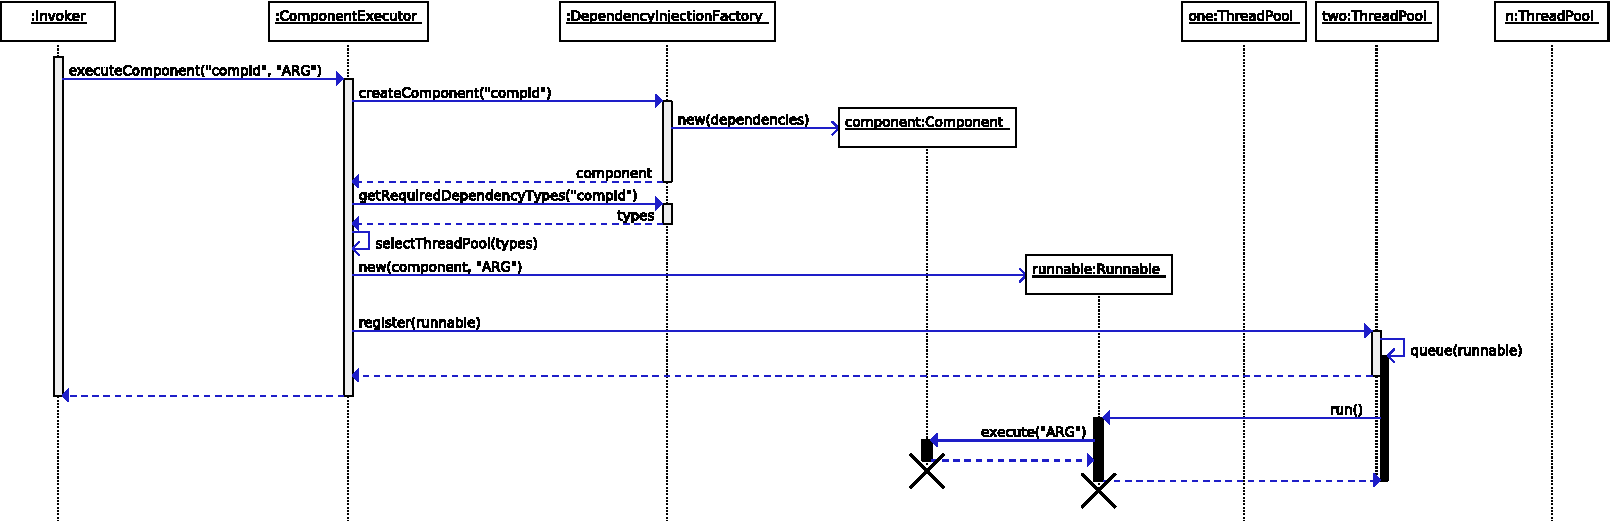
\includegraphics[width=6in]{ExecuteComponentSequenceDiagram}
\caption{Sequence diagram of invoking \texttt{executeComponent(\ldots)}.}
\label{fig:ExecuteComponentSequenceDiagram}
\end{figure}

The prioritisation is achieved by the
\texttt{getRequiredDependencyTypes(\ldots)} method providing the extrinsic
\textsc{dependency injection} \cite{ioc} meta-data for the task
\footnote{\textsc{dependency injection} frameworks using qualification to
identify dependencies of the same type may return a type object containing both
class and qualifier rather than just a class.  The thread pool matching may then
incorporate the qualifier.}.  The developer configures one or more thread pools
responsible for tasks with a particular type of dependency\footnote{Thread pools
may be associated with more than one dependency type.}.  The task is then
matched by its required dependency types (\textsc{categorise task}) to a thread
pool responsible for one or more of its dependency types (\textsc{responsible
team})\footnote{The \texttt{componentId} may also be used for very fine grained
mapping.}.  \texttt{execute(\ldots)} (Listing
\ref{lst:ThreadInjectionInterfaces}) is then invoked by a thread from the
matching thread pool to execute the task (and its contained method). This
provides the necessary isolation of differing tasks for improved tuning of the
server.

For tasks not having dependencies (nor dependencies of any performance
significance), a default thread pool is configured by the developer for their
execution.  This ensures all components are mapped to a thread pool.  It also
means that thread pools need only be configured for dependencies requiring
isolation.

To achieve further efficiencies the implementation of each thread pool may be
specific to its responsible dependency type.  For example, the thread pool may
contain multiple threads for concurrent execution of tasks, a single thread for
serial execution of tasks, or no threads and execute components by borrowing the
thread to reduce thread-context switching (\textsc{do it yourself}).

\texttt{cancel(\ldots)} (Listing \ref{lst:ThreadInjectionInterfaces}) provides
means for the \texttt{TaskExecutor} to cancel the task.
The \texttt{TaskExecutor} will cancel new tasks for a particular thread pool
when queuing the task for a thread will result in exceeding a particular
threshold\footnote{A sufficient threshold would be ensuring the wait time,
determined by a running average of execution time multiplied against the number
of components currently in the queue, is below a certain time.} (\textsc{too
busy}).  Each thread pool may have its own thresholds particular to its
responsible dependency types.  As tasks are mapped to particular thread
pools, this ensures only the appropriate tasks are cancelled.

Once cancelled, the \texttt{TaskExecutor} may discard the task.  The
implementation of the \texttt{can\-cel(\ldots)} method is covered in the
\textsc{escalation} pattern.


\subsubsection*{Consequences}

The isolation provided by using multiple thread pools enables improved tuning of
the server.  Tuning the thread pools (such as restricting the number of threads
or changing the pool's thread nice values) allows prioritising threads and
subsequently prioritising groups of related components.

As each thread pool is executing components for a particular dependency (or set
of dependencies), this allows for adaptive resource management and admission
control regarding the dependency \cite{seda}.  This enables both the number of
threads and dependencies to be dynamically altered to improve throughput.
However, when maximum throughput is reached additional components for execution
above this threshold can be cancelled.

To improve performance of runtime decisions the mapping of component to thread
pool may be cached.  As the dependencies for each component is static, at
application start up time the \texttt{TaskExecutor} may preprocess and
cache the mapping of \texttt{Task} to thread pools to reduce runtime
decision overheads.  This pre-mapping of tasks may also provide warnings
where dependencies of a task make it possible to map the task to
multiple thread pools.  Different conflict mapping resolutions may be employed,
however, ordering the thread pools and assigning tasks based on first match
is a sufficiently adequate algorithm.

For low load servers where a single thread pool is sufficient, having multiple
thread pools can cause increased complexity for developer configuration.  While
this provides the flexibility to focus the tuning of isolated categories of
tasks by tuning their mapped thread pool, it does put the burden on the
developer to understand thread related performance issues (e.g. costs related to
thread stack memory and thread-context switching) and the performance of the
dependencies (along with their related tasks).

The implementation looses its ability to effectively prioritise and cancel tasks
if the task dependencies are too similar.  For example, when used with the
\textsc{thread-per-request} pattern within a web server, all request handling
for dynamic content is likely to use a database connection.  While this will
allow isolation of requests for static content, it will not isolate requests for
dynamic content serviced from cached data rather than database data.  This is
because the request handler (task) will depend on the database connection to
retrieve the data if the data is not cached.  Request handling will, therefore,
need to be segmented into smaller tasks to reduce the occurrences of sets of
common dependencies between tasks, which results in grouping components all onto
the same thread pool.  This is the focus of the collaborating task patterns.


\subsubsection*{Related implementations}

The implementation can be considered a style of cohort scheduling \cite{cohort}
that groups tasks with similar dependencies and infers from that similar
functionality.  However, this implementation works at the application scheduling
level and allows the use of any Operating System thread scheduling algorithms.

The Staged Event-Driven Architecture (SEDA) \cite{seda} provides an
implementation without the use of the \textsc{dependency injection} pattern. 
SEDA directly maps components to a stage and subsequently a thread pool. 
However, the SEDA pipeline has increased thread-context switching as the stage
boundaries are hard, which disallows threads to be borrowed.

Dependency capsules \cite{dependency-capsules} follows the idea of isolating
components that require dependencies to specific thread pools.  However, it
requires a thread-context switch back to a main thread for executing components
without dependencies.

\textbf{TODO:} Go through previous paper and pull in all related implementations. 




\section{Patterns for collaborating tasks}

The following patterns model the collaboration of methods after the way tasks
collaborate within an office.  The implementation notes at the end provide
details on how to implement the patterns.


\subsection{\textsc{\textbf{hand-off}}}

\subsubsection*{Context} Teams hand-off to each other based on the category of
the next task.  For example, after financing a project the finance team would
hand-off to the software development team to build the application.

Method invocations tightly couple the thread of control and disallow changing
the thread of control in invoking another method.

\subsubsection*{Problem} Enable changing the thread of control when invoking another method.

\subsubsection*{Forces} The invoking of a method should still be intuitive for the developer.

\subsubsection*{Solution}  Provide an interface as a parameter to method.  The
interface will have a proxy implementation that has its methods asynchronously
invoke the respective target methods.

\subsubsection*{Consequences} Able to invoke the target method by another thread of control.

No return value will be available from the invoked method due to the
asynchronous invocation.

Each hand-off will incur the cost of a thread context-switch.

\subsubsection*{Related Patterns}



\subsection{\textsc{\textbf{escalation}}}

\subsubsection*{Context} Within an office a person will escalate issues to their
manager.  However, for a method the exception from a method is thrown to the
invoking method.

\subsubsection*{Problem} Escalate an exception to a manager rather than the caller.

\subsubsection*{Forces} Method exceptions follow the thread of control's stack
back to an appropriate \texttt{try~\ldots~catch} block for handling the
exception.

\subsubsection*{Solution} Intercept the exception and \textsc{hand-off} to a
manager handling method for the exception.

\subsubsection*{Consequences} Caller does not deal with exceptions from
\textsc{hand-off} method invocations.  This does mean the caller will not be
aware of failures in its invoked methods.  It is, however, unreasonable to have
the caller responsible for all downstream issues in the process flow.

\subsubsection*{Related Patterns} \textsc{hand-off} is used to enable the
exception to be asynchronously handled by another method.



\subsection{\textsc{\textbf{define process flows}}}

\subsubsection*{Context} The process within an office is a sequence of tasks
where the next task depends on what occurs with the current task.  The process
can be changed by altering the next task for each outcome of the current task.

Method invocation prevents this flexibility as the methods must be altered to
change the sequence of method execution.

\subsubsection*{Problem} Provide change in execution order of methods without
requiring to change the methods.

\subsubsection*{Forces} Method invocation is tighlty coupled at the code level.

\subsubsection*{Solution} Use \textsc{hand-off} and, via configuration, map the
hand off interface method to trigger the execution of the target method. 
Furthermore, provide an implicit hand-off on completion of a method to execute a
next method if no other hand-off is triggered.

\subsubsection*{Consequences} Configuration maps the flow of methods rather than
being hard-coded within the method.

The indirection will make it difficult to follow the flow of the process.  The
configuration, however, is represented graphically to make it easier and more
intuitive to follow.

\subsubsection*{Related Patterns} \textsc{hand-off} is used to enable the
indirection for configuration mapping of hand-offs and to handling methods.



\subsection{\textsc{\textbf{do your work}}}

\subsubsection*{Context} Within the process flow a team may be assigned to
execute a sequence of tasks. Rather than passing the tasks around to different
people in the team, it is more efficient for one person to complete the tasks
without the cost of hand-offs.

\subsubsection*{Problem} Use the same thread to execute the sequence of methods
when the methods hand-off back to the same thread pool to avoid excessive
thread-context switching.

\subsubsection*{Forces} The \textsc{hand-off} is asynchronous.

\subsubsection*{Solution} Before the asynchronous hand-off, check if the thread
for the next method is of the same responsible thread pool and if so execute the
next method synchronously (i.e. with the current method's thread of control).

\subsubsection*{Consequences} Thread context-switching is reduced for sequential
methods of the same responsible thread pool.

\subsubsection*{Related Patterns} Is a sequence on \textsc{hand-off} to reduce
thread context switching.



\subsection{\textsc{\textbf{wait to proceed}}}

\subsubsection*{Alternate name} Future \textbf{TODO: find reference}.

\subsubsection*{Context} Need to know when the hand-off task (and further
handed-off tasks by that task) is complete.

\subsubsection*{Problem}

\subsubsection*{Forces}

\subsubsection*{Solution}

\subsubsection*{Consequences}

\subsubsection*{Related Patterns}



\subsection{\textsc{\textbf{pick up task again}}}

\subsubsection*{Alternate name}

\subsubsection*{Context} Trigger a hand-off and come back to current task again
when the hand-off tasks complete.

\subsubsection*{Problem}

\subsubsection*{Forces}

\subsubsection*{Solution}

\subsubsection*{Consequences}

\subsubsection*{Related Patterns}



\subsection{\textsc{\textbf{record information}}}

\subsubsection*{Alternate name} \textsc{flyweight}~\cite{gof}.

\subsubsection*{Context} With an office information is recorded so that later
tasks can retrieve this information.

Methods, however, may only use the arguments supplied from the calling
method\footnote{The method may also access implicit references via its
owning object}.

\subsubsection*{Problem} The method being able to retreive information from
previous methods other than just its calling method.

\subsubsection*{Forces} Method invocation requires the caller to provide all
parameters to the invoked method.

\subsubsection*{Solution} Use \textsc{dependency injection}~\cite{ioc} to inject
cached dependencies as the arguments to the method.

\subsubsection*{Consequences} As the dependencies provide cached state, they
allow all downstream methods to retrieve the state.

Making the dependency state mutable allows further downstream methods awareness
of changes in information as the tasks in the process execute.

\subsubsection*{Related Patterns} Is a sequence on \textsc{dependency
injection}~\cite{ioc} to cache dependencies and inject them as arguments to the
method.



\subsection{\textsc{\textbf{inbox}}}

\subsubsection*{Alternate name} Future \textbf{TODO: find reference}.

\subsubsection*{Context}

\subsubsection*{Problem}

\subsubsection*{Forces}

\subsubsection*{Solution}

\subsubsection*{Consequences}

\subsubsection*{Related Patterns}



\subsection{Implementation of the task collaboration patterns}

\subsubsection*{Background}

Both the \textsc{thread-per-request} pattern \cite{thread-per-request} (basis of
many mainstream web servers\footnote{For popular web servers (Netcraft November
2012 survey) dynamic web content is serviced by CGI/FastCGI with for example PHP
scripts, Microsoft's HTTP.sys/WAS, and JEE Servlets.}) and the \textsc{proactor}
pattern \cite{proactor} (basis of event-driven web servers) impose tight
coupling on the collaboration of components (objects wrapping the execution of a
method).  The \textsc{thread-per-request} pattern enables invoking components by
synchronous methods, which is intuitive for developers \cite[p. 2]{proactor}. 
In contrast, the \textsc{proactor} pattern enables asynchronously invoking a
constructed component by registering it for execution by another thread of
control (allowing to execute components concurrently).  In both patterns, they
tightly couple the collaboration of components as the
\textsc{thread-per-request} pattern must have the invoker provide the thread of
control and the \textsc{proactor} pattern must have the invoker construct the
invoked component.

The \textsc{thread-per-request} pattern imposes a synchronous interface that
prevents asynchronous use of components.  As the number of downstream systems
increases from a typical single database to a variety of services (e.g.
reverse 10K problem \cite{reverse-ten-k-problem}), the
\textsc{thread-per-request} pattern requires the developer to manually handle
the multi-threading issues involved in the concurrent communication to
downstream systems to efficiently service a request.  It is, therefore, better
to use the \textsc{proactor} pattern in this circumstance.

The \textsc{proactor} pattern requires increased coding by the developer to
invoke a component.  To invoke a component, the developer must construct the
component, register it for execution, and then handle completion of the
component.  Furthermore, handling completion of multiple concurrently executing
components may not be intuitive for many developers.  When concurrency is not
necessary, using methods to synchronously invoke components via the
\textsc{thread-per-request} pattern can produce less code that will likely be
more intuitive for developers.  Therefore, invoking components should be via a
method invocation for potentially less code and easier understanding of the
code.

The synchronous nature of the \textsc{thread-per-request} pattern also imposes
constraints on the order in which the components are executed.  Within the
\textsc{thread-per-request} pattern, the sequence in which the components are
executed is dictated by synchronous direct method calls.  As a result, the
\textsc{thread-per-request} pattern provides little indirection to invert the
control over the order components are executed unless components match on method
signatures.

The \textsc{proactor} pattern also imposes hard-coded order over the components
invoked (albeit they may end up being executed concurrently).  The invoker must
construct the component to be asynchronously invoked and therefore this does not
provide the indirection to control invoking a different component.

The \textsc{thread-per-request} pattern and \textsc{proactor} pattern further
tightly couple invoking a component by the invoker being required to handle
possible exceptions.  The invoker may not be appropriately responsible to handle
a resulting exception and this should be delegated to another component.

Loosely coupling the invocation of components leads to better re-use of
components.  ``Tight coupling leads to monolithic systems, where you can't
change or remove a \ldots [component] without understanding and changing other
\ldots [components]'' \cite[p. 24-25]{gof}.  Having to change components to
invoke them restricts the ability to re-use the components.

For a framework (e.g. web server) to extend itself by invoking components, the
framework pre-defines the component's interface to enable invoking it.  However,
components should be able to invoke other components for re-use of the
component.  To enable re-use of these components the interface to invoke
components should be standardised.


\subsubsection*{Implementation}

On executing a component, provide the \texttt{ComponentContext} (Listing
\ref{lst:ContinuationInjectionInterfaces}) to the component.  The
\texttt{ComponentContext} contains a mapping of \texttt{continuationId} to a
handling component.  As each mapping is a continuation (''goto'' for executing a
component), this allows injecting the necessary continuations into the
component.

The \texttt{ComponentContext} for a component is constructed via a
\texttt{ComponentContextFactory} (Listing \ref{lst:ContinuationInjectionInterfaces})
to keep the continuation mapping configuration centrally managed.  This is
similar to the \texttt{DependencyInjectionFactory} (Listing
\ref{lst:ContinuationInjectionInterfaces}) containing centrally managed
configuration to create dependencies.

\lstset{caption=\textsc{continuation injection} pattern interfaces\protect\footnotemark.}
\begin{lstlisting}[float,label=lst:ContinuationInjectionInterfaces]

    interface Component {
        void execute(ComponentContext context);
        String[] getContinuationIds();
        String[] getStateIds();
    }

    interface ComponentContext {
        Object getState(String stateId);
        Future doContinuation(String continuationId, Object parameter);
        void handleException(Exception exception);
        void continueComponent();
    }
    
    interface ContinuationInjectionFactory {
        ComponentContext createComponentContext(String componentId
                                               , Object parameter
                                               , DependencyContext context);
    }
    
    interface DependencyInjectionFactory {
        DependencyContext createDependencyContext();
    }
    
    interface DependencyContext {
        Object getDependency(String dependencyId);
    }
\end{lstlisting}
\footnotetext{A rudimentary example implementation of the
\texttt{DependencyInjectionFactory} is wrapping Spring's \cite{spring}
\texttt{BeanFactory} to create an implementation of \texttt{DependencyContext}
by it obtaining (and caching) the calling of Spring's \texttt{getBean(\ldots)}
method.  A more functional example implementation would utilise Spring's
\texttt{ApplicationContext} as the \texttt{DependencyContext} to manage the
context for the components and their dependencies.}

The \textsc{continuation injection} pattern provides algorithms which implement the
\textsc{proactor} pattern's Proactor Initiator, Asynchronous Operation and
Completion Dispatcher/Handler participants.  The continuation triggers the
Proactor Initiator to register an Asynchronous Operation containing the desired
component for execution.  The Completion Dispatcher/Handler is also registered
and notifies the Proactor Initiator when the Asynchronous Operation completes.
Using a Proactor Initiator per request to track completion of Asynchronous
Operations (components) allows a response to be provided once all components for
the request are completed.

The components are constructed via the \textsc{dependency injection} pattern
\cite{ioc}.  The \texttt{Dependency\-InjectionFactory} (Listing
\ref{lst:ContinuationInjectionInterfaces}) centrally manages the dependency
configuration and creates a \texttt{Depend\-ency\-Context} that constructs and
caches dependency instances for the components.  The
\texttt{Dependency\-Context}, that manages the life-cycle of dependencies, is
aligned to the Proactor Initiator life-cycle.  This allows for both the
dependencies of the components and the components themselves to be specific to
the request being serviced.  It also allows the state/resources within these
dependencies to be managed within the life-cycle of servicing the request.

Re-using dependencies between components allows sharing state between the
components.  For the \textsc{thread-per-request} pattern, the method signature
tightly couples sharing state by requiring particular parameters and by only
providing a single return value.  For the \textsc{proactor} pattern, the invoker
must have all state available to construct the Asynchronous Operation and
Completion Dispatcher/Handler which tightly couples the invocation.  Providing
mutable state within dependencies that are re-used across components allows
components to share state.  This is similar to a \textsc{thread-per-request} web
server that shares state between components by attributes (dependencies) within
request, session and application scopes.  To further decouple the component from
global dependency identifiers the \texttt{ComponentContext} contains a mapping
of \texttt{stateId} to \texttt{dependencyId} to allow the component to obtain
the extrinsically defined \textsc{dependency injection} dependencies via the
\texttt{getState(\ldots)} method (Listing
\ref{lst:ContinuationInjectionInterfaces}).  The invoking component only needs
the dependencies (state) it requires and is not coupled to the invoked component
by having to provide the entire set of dependencies (state) for the invoked
component.

The \texttt{doContinuation(\ldots)} method (Listing
\ref{lst:ContinuationInjectionInterfaces}) allows a component to invoke another
component.  As the \texttt{continu\-ationId}s are static for each component,
developer configuration provides the continuation mapping to the respective handling
component.  The method does allow one argument to be passed to the invoked
component.  This is for more intuitive development by associating the invocation
with passing state.  If multiple arguments are required, they should be
encapsulated into an object for passing.  To maintain loose coupling, the
invoked component obtains the argument as state (i.e. \texttt{getState(\ldots)}
method in listing \ref{lst:ContinuationInjectionInterfaces}) so the invoked
component need not differentiate between dependencies and parameters.  The
invoked component may also ignore the continuation argument should it not depend
on it.  Figure \ref{fig:DoContinuationSequenceDiagram} provides a sequence
diagram of invoking a component via the \texttt{doContinuation(\ldots)} method.
  
\begin{figure}[!t]
\centering
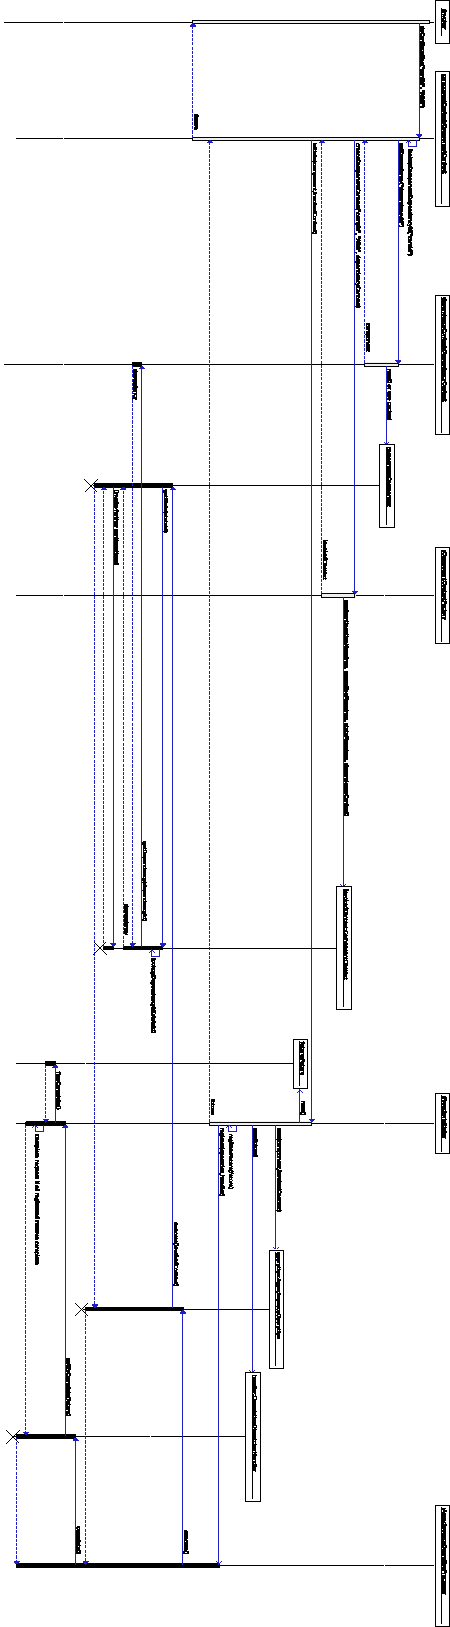
\includegraphics[height=7.4in]{DoContinuationSequenceDiagram}
\caption{Sequence diagram of invoking \texttt{doContinuation(\ldots)}.}
\label{fig:DoContinuationSequenceDiagram}
\end{figure}
 
As the \texttt{doContinuation(\ldots)} method asynchronously invokes the
component, the returned \texttt{Future} is used to determine when the potential
tree of invoked components has completed.  The \texttt{Future} utilises the
Proactor Initiator's tracking of Asynchronous Operation completion to determine
when the tree of Asynchronous Operations realising the continuation has
completed.  This enables process continuations \cite{process-continuation} to be
spawned by repeatedly calling \texttt{doContinuation(\ldots)}.  The process
continuations aid in resolving the reverse 10K problem
\cite{reverse-ten-k-problem} by executing multiple components concurrently.
Also, as state is shared by dependencies, the \texttt{Future} does not provide a
return value.  This further decouples the invocation as the invoking component
is not tightly coupling the expected return type for the invocation.

Exceptions from the methods are handled by being mapped to a
\texttt{continuationId}.  The component invokes the
\texttt{handle\-Excep\-tion(\ldots)} method with the exception\footnote{For
easier development of components, the component's \texttt{execute(\ldots)}
method signature may allow throwing the exception which is caught by a wrapping
executor that calls the \texttt{handleException(\ldots)} method with the caught
exception.}.  The \texttt{handleException(\ldots)} method is implemented by
mapping the exception type to a \texttt{continuationId} and invoking the
\texttt{doContinuation(\ldots)} method with the exception as the argument. 
Continuations for specific exception types of the component may be configured by
the developer.  The developer will also configure ''catch all'' continuations
for the application to handle exceptions from any component to ensure all
exceptions are handled (e.g. handling of the runtime non-checked exceptions). 
This allows default handling of exceptions within the application and gives the
component the ability to override only as necessary.  This is similar to
\texttt{catch} blocks for handling exceptions at different levels of the method
call hierarchy.  It also reduces the configuration for developers by only having
to provide the overriding exception handling configuration for components.  The
invoking component is, therefore, decoupled from handling the invoked
component's exceptions, as the exceptions are handled by other components.

The \texttt{continueComponent()} method (Listing
\ref{lst:ContinuationInjectionInterfaces}) enables re-executing the current
component.  The Proactor Initiator may be implemented to defer the execution of
a component again until invoked continuations by the component are completed. 
The Proactor Initiator uses the same tracking of completion as the
\texttt{Future} to determine the completion of the last Asynchronous Operation
(component) for the invoked continuations.  On completion of the last
Asynchronous Operation, the Proactor Initiator registers the component within an
Asynchronous Operation for execution again.  This, for example, allows deferring
the execution of the component until an invoked Operating System asynchronous
I/O operation completes - a key aspect of the \textsc{Proactor} pattern for
improved concurrency.

The execution of a continuation may also be deferred until all other
continuations from the component are complete.  Each continuation mapping
contains a configurable attribute to delay invoking the handling component
until all other invoked continuations for the component are complete.  This
avoids the developer having to provide additional code to check the completion
of the \texttt{Future}s for all concurrently executed continuations (i.e.
continuations not flagged to wait) before proceeding with the desired
continuation.  Should the component invoke multiple continuations configured to
wait, these continuations will be executed one after the other as each is
completed.  This further decouples the invocation as deciding on whether to wait
on the completion of a continuation can be undertaken by configuration outside
the component.

The intuitiveness of sequential programming is maintained by using implicit
continuations \cite{continuations} to sequentially chain components.  Each
\texttt{ComponentContext} also maintains an optional implicit continuation. 
Should no continuation be invoked (i.e. \texttt{doContination(\ldots)} method
invoked or an exception thrown) the implicit continuation is invoked on
completion of the component.  This allows chaining together components to be
executed sequentially.

While the \textsc{proactor} pattern focuses on asynchronous interaction between
Asynchronous Operations, the \texttt{ComponentContext} does not restrict the
servicing of the continuation invocation from being synchronous.  In cases where
it is more efficient to synchronously invoke the component and avoid the
thread-context switching overheads, this can be controlled by the developer with
a flag in the continuation mapping configuration.  When the continuation is
flagged for synchronous execution, the Proactor Initiator synchronously executes
the component within the thread of control invoking the
\texttt{doContinuation(\ldots)} method.  In this case, the Proactor Initiator
does not wrap the component in an Asynchronous Operation for asynchronously
execution.  Having the configuration option for developers to control borrowing the
thread of control further loosely couples invocation of components, as invoked
components may be more efficiently executed by the same thread of control (e.g.
when retrieving data from an in memory cache).

To ease developer understanding of the collaboration between components, the
mapping configuration of \texttt{continuationId}  to \texttt{componentId} may be
graphical.  Developer tools will use the \texttt{getContinuationIds()} method
(Listing \ref{lst:ContinuationInjectionInterfaces}) to obtain the list of possible
continuations for a component.  The tools then graphically represent the
components as nodes with the continuation mappings being directed lines between
these nodes.  Due to the similarity of this configuration with service
orchestration, this graphical configuration is identified as Component
Orchestration\footnote{Component orchestration may also be identified as
function, procedure, method or operation orchestration depending on the
implementing language.}.  The \texttt{stateId} to \texttt{dependencyId} mapping
for a component may also be included in this configuration by dependencies
represented as further nodes to be linked to \texttt{stateId} anchors on the
components.  The developer tools use the \texttt{getStateIds()} method (Listing
\ref{lst:ContinuationInjectionInterfaces}) to obtain the list of possible state
objects required for the component\footnote{The \texttt{getContinuationIds()}
method may be enhanced to also return the argument types that the component will
provide on each of the continuations.  The \texttt{getStateIds()} may also be
enhanced to provide the expected type the component requires for each
\texttt{stateId}.  Providing this type information allows the continuation
argument to be type validated against the handling component's required
parameter state type to reduce runtime errors and therefore may restrict some
mapping changes.  However, an adapting component may be mapped in between to
remove this restriction by transforming the argument to the necessary type for
the handling component.}.


\subsubsection*{Example}

Listing \ref{lst:Example_Method_Operation} shows the example developer
implementation code.  A generic component implementation is used to reflectively
invoke the \texttt{retrieveData(\ldots)} method. It will:
\begin{enumerate}
  \item Obtain an instance of the \texttt{CacheOperation} via the \texttt{getState(\ldots)} method.
  \item Obtain both the \texttt{key}\footnote{\texttt{key} is a continuation argument from the previous component.} and \texttt{cache} again via the \texttt{getState(\ldots)} method.
  \item Instantiate a proxy implementation of the \texttt{CacheContinuation} interface that implements the \texttt{cacheMiss(\ldots)} method by invoking the \texttt{doContinuation(\ldots)} method. 
  \item Reflectively invokes the \texttt{retrieveData(\ldots)} method with the above arguments.
\end{enumerate}

\lstset{caption=Example developer implementation code for a component\protect\footnotemark}
\begin{lstlisting}[float,label=lst:Example_Method_Operation]

  interface CacheContinuations {
    void cacheMiss(String key);
  }

  class CacheOperation {    
    public Data retrieveData(String key, Cache cache
                            , CacheContinuations continuations
                            ) throws IOException {
        Data data = cache.get(key);
        if (data == null) {
            continuations.cacheMiss(key);
            return null; // finish operation
        }
        return data;
    }
  }
\end{lstlisting}
\footnotetext{\texttt{retrieveData} may also be a function should the implementing programming language support functions.}

Continuations from the \texttt{retrieveData(\ldots)} method are:
\begin{itemize}
  \item \texttt{cacheMiss(\ldots)} which is mapped to \texttt{Retrieve data from database}.
  \item Implicit continuation which is mapped to the \texttt{Render HTTP response}\footnote{The return value from the method is used as the continuation argument.}.
  \item \texttt{IOException} which is mapped to a component providing an error message page.  It may also be mapped to \texttt{Retrieve data from database} to attempt to continue servicing the request.
\end{itemize}


\subsubsection*{Consequences}

The mapping of \texttt{continuationId} to \texttt{componentId} (component) is
contained within configuration.  This enables changing the handling component
without changing the code of the components.  Changing the handling component
enables re-ordering the chained sequence of components that are executed to
service a request.

Using the \texttt{doContinuation(\ldots)} method to invoke components, with the
invoked component using implicit continuations to further invoke other
components, is similar to spawning threads.  The continuations result in the
concurrent execution of sequential chains of components.  This allows for the
intuitiveness of the \textsc{synchronous multi-threaded} pattern \cite{proactor}
for handling concurrency.

Without the graphical configuration of Component Orchestration, understanding
the collaboration of components would become difficult due to the indirection
involved.  This is especially relevant when components are implemented as
methods, which can result in a large number of components needing to
be configured together\footnote{Future work will present the patterns
OfficeFloor \cite{officefloor} uses to encapsulate Component Orchestration
configuration for re-use to avoid its graphical representation from becoming
unwieldy.}.

As components are being executed asynchronously (potentially by different
threads of control), using debugging developer tools to step through the
execution of servicing a request will involve stepping through the implementing
code of the \texttt{ComponentContext}.  This can distract developers and can
make it difficult to trace the execution as it switches between threads. 
However, debugging tools can be enhanced/configured to automatically skip over any
instructions of the \texttt{ComponentContext} implementation to avoid this
distraction.

Furthermore, as components are potentially executed by different threads of
control, the stack trace automatically provided by the
\textsc{thread-per-request} pattern no longer reflects the call hierarchy for
servicing a request.  This can make it more difficult to debug issues.  However,
the Proactor Initiator may be flagged to record the tree of components invoked
so that the tree can be traversed back to the root to identify the sequence of
continuations to the component throwing the exception.  The whole tree can also
be reported to aid the developer in debugging the cause of the issue.

Integrating the \textsc{continuation injection} pattern with code not contained
in components does not allow access to the \texttt{ComponentContext} to invoke
the continuation for the first component.  Listing
\ref{lst:ContinuationInjectionInterface} provides an interface that allows code
not contained in a component to invoke the first continuation.  The returned
\texttt{Future}, from the Proactor Initiator tracking of Asynchronous
Operations, indicates when all components are complete.  To retrieve results,
the \texttt{parameter} would be used as a visitor (\textsc{visitor} pattern
\cite{gof}) and be loaded with results by the invoked components.

\lstset{caption=Interface for code not within a component to invoke a continuation.  The component for the continuation is identified with the \texttt{componentId} parameter.}
\begin{lstlisting}[float,label=lst:ContinuationInjectionInterface]

    interface ContinuationInjection {
        Future doContinuation(String componentId, Object parameter);
    }
\end{lstlisting}

When implementing components with functions, the functions will not be pure.  As
state is shared between components by mutable state within dependencies,
functions will need to cause side effects (mutate state) to share state with
other components (functions).  Therefore, caution is required in developing a
component to ensure it is not coupled to other components by expectations of
particular mutations in state.  This is necessary to avoid invalid side effects
due to changes in configuration that results in re-ordering the execution of the
components.


\subsubsection*{Related implementations}

This provides an implementation of the Actor Model \cite{actors} as it adheres
to the principles of the Actor Model.  The component is the actor.  The
asynchronous communication between components decouples the continuation
argument (message) from the sending component (actor).  The \texttt{componentId}
provides an address for a component (actor).  The provided
\texttt{continuationId}s restricts the components (actors) that may be used.

The implementation can also be considered a form of continuation-passing style
\cite{continuations} except that the continuation is injected rather than passed
as a parameter.  The added benefit of injecting the continuation is that the
component is free to depend on as many continuations as necessary.  It also
means that as the application evolves the component encapsulates potential
changes requiring different continuations.  The indirection allows managing
these changes as configuration changes rather than code changes.

\textbf{TODO:} see preious paper for further related implementations.



\section{Patterns for re-use of Tasks (\textsc{method inversion of control})}


\subsection{\textsc{\textbf{task defines itself}}}

\subsubsection*{Alternate name}

\subsubsection*{Context}

\subsubsection*{Problem}

\subsubsection*{Forces}

\subsubsection*{Solution}

\subsubsection*{Consequences}

\subsubsection*{Related Patterns}



\subsection{\textsc{\textbf{use proven tasks}}}

\subsubsection*{Alternate name}

\subsubsection*{Context}

\subsubsection*{Problem}

\subsubsection*{Forces}

\subsubsection*{Solution}

\subsubsection*{Consequences}

\subsubsection*{Related Patterns}



\subsection{\textsc{\textbf{process defines itself}}}

\subsubsection*{Alternate name}

\subsubsection*{Context}

\subsubsection*{Problem}

\subsubsection*{Forces}

\subsubsection*{Solution}

\subsubsection*{Consequences}

\subsubsection*{Related Patterns}



\subsection{Implementation of task re-use patterns}

\subsubsection*{Background}

Applications built with \textsc{layers} typically impose a top-down approach to
design.  ``The \textsc{layers} require and provide \textsc{explicit interfaces}
from and to each other, in a top-down manner, from the higher to the lower
\textsc{layers}'' \cite[p. 11]{ioc}.  The higher-level layer components (object
that wraps a method) define the variation points that are ``predefined points in
the control and data flow which allow for modifying and extending a component's
behaviour'' \cite[p. 5]{ioc}.  A top-down approach is required, as the
higher-level layers control what variation points may be implemented by the
lower-level layer components.

Inverting the control by allowing the lower-level layer components to control the
variation points to be implemented by the higher-level layer components provides
inversion of control.  Inversion of control occurs by inverting the top-down
control in designing applications to be bottom-up control.  This bottom-up
control allows the application architecture to be evolved upwards. Therefore,
\textsc{method inversion of control} better suits development methodologies, such as
Agile, that evolve application architectures upwards.

The components need to be composed within an architecture that is dictated by
the framework.  The framework ``will define the overall structure, its
partitioning into \ldots [components], the key responsibilities thereof, how the
\ldots [components] collaborate, and the thread of control'' \cite[p.26]{gof}.
Using the components within a framework, therefore, identifies the following
requirements of a component's \textsc{explicit interface}:
\begin{itemize}
  \item components must have a key responsibility;
  \item components must be able to collaborate with other components; and
  \item components require a thread of control.
\end{itemize}

The collaboration of components can further be defined as the following
requirements:
\begin{itemize}
  \item components must be able to invoke other components;
  \item components must be able to share state; and
  \item exceptions from components need to be handled.
\end{itemize}

Within frameworks, the method/function signature is the interface between
components.  ``The set of all [method] signatures defined by an object \ldots
characterizes the complete set of requests that can be sent to the object''
\cite[p. 13]{gof}.  As frameworks are composed of objects (and possibly
functions), the method/function signature defines the interface between
objects/functions and subsequently components.

The method/function signature meets the requirements as it:
\begin{itemize}
  \item has a key responsibility identified by its name;
  \item may invoke other methods/functions;
  \item shares state with other methods/functions by arguments and return values;
  \item provides declaration of exceptions for handling; and
  \item can be executed by the thread of control\footnote{For a stateless component interface, thread local variables are to be avoided to not incur affinity to a thread.}.
\end{itemize}

The method/function interface is, however, subject to tight coupling.  The tight
coupling occurs from the invoking higher-level layer component having to:
\begin{itemize}
  \item define the method/function name;
  \item provide the necessary arguments;
  \item possibly use the return value;
  \item handle potential exceptions; and
  \item provide the thread of control to execute the method/function.
\end{itemize}

This tight coupling imposed by the method/function results in the hierarchical
\textsc{layers} architecture where variation points (\textsc{explicit
interfaces}) are controlled by the higher-level layers.  The higher-level layer
component provides a \textsc{template method} \cite{gof} which is the variation
point that lower-level layer components may extend through inheritance
(\textit{abstract classes}) or collaboration (\textit{interfaces}).

Within a \textsc{layers} architecture having variation points defined by
\textsc{template method}s requires refactoring of the \textsc{template method}
to increase the variability of the lower-level layer components.  Increasing the
variability ``requires adapting the \textsc{explicit interfaces} between the
\textsc{layers} to stipulate the types of variation parameters'' \cite[p.
5]{ioc} to allow control over the lower-level layers by the higher-level layers.

Instead of attempting to define variation points at the higher-level layers to cover
all possible variations of the lower-level layers, control should be inverted and
given to the lower-level layers to define the variation points.  However, given
that \textsc{template methods} impose a top-down control over variation points,
another form of \textsc{explicit interface} is necessary for lower-level layer
components to provide bottom-up control over defining variation points for the
application.


\subsubsection*{Implementation}

Use \textsc{dependency injection}, \textsc{thread injection} and
\textsc{continuation injection} to have the lower-level layer component control
its required variation points.

\textsc{dependency injection} \cite{ioc} (used within \textsc{continuation
injection}) enables the lower-level layer component to specify the state
(objects) it requires.  When \textsc{dependency injection} is used within
\textsc{continuation injection}, the lower-level layer component specifies its
required state (objects) via \texttt{stateId}s.  As the lower-level layer
retrieves its state from \textsc{dependency injection}, the invoking
higher-level layer components need only provide the single optionally used
argument.  This allows the lower-level layer component to specify as many
dependencies as is necessary.  It, therefore, gives the lower-level layer component
control over what state (objects/dependencies) it may depend on.

\textsc{thread injection} enables the lower-level layer component to specify its
thread of control.  By the the lower-level layer component having control over
specifying its required dependency types, the lower-level layer component may
specify additional dependencies to control which thread pool will be used to
execute it.

\textsc{continuation injection} enables the lower-level layer component to
specify its required collaboration by \texttt{componentId}s.  The mapping of
\texttt{continuationId} to \texttt{componentId} enables configuring the
higher-level layer components for handling each required continuation by the
lower-level layer component.  As the invoking higher level-layer component does
not need to provide references to these handling components on invoking the
lower-level layer component, the lower-level layer component may specify as many
continuations as are necessary for its required collaboration variation points. 
This gives the lower-level layer component control over its collaboration
variation points.

Exceptions from components are handled by \textsc{continuation injection}.  The
exception is mapped to a \texttt{continuationId} and subsequently mapped to a
handling component.  As the  invoking higher-level layer component is decoupled
from having to handle the exceptions, the lower-level layer component is free to
control throwing as many exceptions as is warranted.

Using the \textsc{dependency injection}, \textsc{thread injection} and
\textsc{continuation injection} patterns together provides the necessary inversion
of control over variation points as the lower-level layer component controls:
\begin{itemize}
  \item its name (\texttt{componentId}) which is decoupled from the invoking higher-level layer component invocation (\texttt{contin\-uationId}) by \textsc{continuation injection};
  \item which invocations (\texttt{continuationId}s) are necessary via \textsc{continuation injection};
  \item what state (\texttt{stateId}s) is required by \textsc{dependency injection};
  \item the types of exceptions that may be thrown by \textsc{continuation injection}; and
  \item the thread of control by \textsc{thread injection}.
\end{itemize}

Therefore, the \texttt{Component} interface (Listing
\ref{lst:IocInjectionInterfaces}) is the \textsc{explicit interface} for
lower-level layer components to control the variation points of the application.
 The component is executed by the \textsc{thread injection} pattern's
\texttt{ComponentExecutor} after creation by the \textsc{continuation injection}
pattern's \texttt{ComponentContext}.  As \textsc{continuation injection} and
\textsc{thread injection} share the same \texttt{DependencyInjectionFactory},
the \textsc{thread injection}'s \texttt{ComponentExecutor} trusts the
\textsc{continuation injection} pattern to pass the component within the
\texttt{Runnable} for execution.  The \texttt{Runnable} is constructed by the
\textsc{continuation injection} pattern and contains the Asynchronous Operation
to execute the component and the Completion Handler/Dispatcher to flag the
\texttt{Future} complete.  The cancellation exceptions of the \textsc{thread
injection} pattern (i.e. \texttt{cancel(\ldots)} method of listing
\ref{lst:ThreadInjectionInterfaces}) are handled by the
\texttt{handleException(\ldots)} method to enable application level handling of
overload conditions.  The \texttt{ComponentContext} (constructed by the
\texttt{ComponentContextFactory}) provides means to retrieve state via the
\textsc{dependency injection} \texttt{Dependency\-Context} and to invoke other
components via \textsc{continuation injection}.

\lstset{caption={Combined \textsc{thread injection}, \textsc{continuation injection} and \textsc{dependency injection} pattern interfaces\protect\footnotemark.}}
\begin{lstlisting}[float,label=lst:IocInjectionInterfaces]

    interface Component {
        void execute(ComponentContext context);
        String[] getContinuationIds();
        String[] getStateIds();
    }

    interface ComponentContext {
        Object getState(String stateId);
        Future doContinuation(String continuationId, Object parameter);
        void handleException(Exception exception);
        void continueComponent();
    }
    
    interface ContinuationInjectionFactory {
        ComponentContext createComponentContext(String componentId
                                               , Object parameter
                                               , DependencyContext context);
    }
    
    interface DependencyInjectionFactory {
        Type[] getRequiredDependencyTypes(String dependencyId);
        DependencyContext createDependencyContext();
    }
    
    interface DependencyContext {
        Object getDependency(String dependencyId);
    }
    
    interface Runnable {
        void run();
        Component getComponent();
        ComponentContext getComponentContext();
    }

    interface ComponentExecutor {
        void executeComponent(String componentId 
                             , Runnable runnable);
    }
\end{lstlisting}
\footnotetext{Integer identifiers may be used for fast array look ups rather than strings.}


\subsubsection*{Implicit Thread}

Implicit threads may be used to reduce the thread-context switching of the
\textsc{inversion of control} pattern.

The continuation may borrow the thread of the invoking component if it results
in being executed by the same thread pool.  The \textsc{proactor} pattern
stipulates that Asynchronous Operations (components) ``must be performed without
borrowing the application's thread of control'' \cite[p. 8]{proactor}.  The
borrowing of the thread is the focus of the \textsc{reactor} pattern
\cite{reactor}.  Rather than dispatching back to the same thread pool, the
continued component may borrow the thread to avoid the overhead of a
thread-context switch.

Borrowing the thread of control can also be extended to the default thread pool
for the \textsc{thread injection} pattern.  Components mapped to the default
thread pool do not have dependencies requiring isolation.  As these components
do not require isolation, they are more efficiently executed by borrowing the
thread rather than incurring the cost of a thread-context switch.

The borrowed thread is the implicit thread.  Like an implicit continuation that
executes the next operation \cite{continuations}, the implicit thread executes
the next component unless an explicit thread is required.  This can result in
a server servicing the entire request without a thread-context switch
should all the components involved not require an explicit thread
(e.g. web page content obtained from cache).

An implicit thread has similarities to a monadic thread \cite{monadic-thread}.
The components can be considered nodes in the lazy trace of the monadic thread.
The advantage of an implicit thread\footnote{Beyond Component Orchestration
being easier for the developer to understand than monad programming.} is that
\textsc{thread injection} pattern allows the execution of blocking I/O nodes
(components) to be prioritised by using explicit threads.  Monadic threads can
not prioritise blocking I/O nodes as they know little about them and
subsequently execute them within a single thread pool.


\subsubsection*{Consequences}

Using \textsc{inversion of control} allows bottom-up control over the design of
the application.  As the variation points are controlled by the lower-level
layer components, developers may start by building the lower-level layer
components first.  As the lower-level layer components are less abstract, the
developer is able to focus on more concrete problems and provide only the
necessary variation points to solve the particular problem.  This avoids over
engineering the design of the application.  Furthermore, as the higher-level
layer components are built last, there is less need for large initial top-down
designs.

\textsc{method inversion of control} also enables bottom-up evolution of the
application.  Within applications imposing top-down design, the
\textsc{explicit interface} (\textsc{template method}) between \textsc{layers}
needs to be refactored to account for required changes to increase the
variability of the lower-level layer components as the application evolves
\cite{ioc}.  Within bottom-up \textsc{inversion of control}, the lower-level
layer component may introduce new variation points that are implemented by
higher-level layer dependencies and components.  As the \textsc{explicit
interface} to invoke the lower-level layer component does not change, the
invoking higher-level layer components do not require refactoring to evolve the
application.

Within \textsc{method inversion of control}, object-orientation provides the
implicit state (dependencies) to a component.  When a method is used as the
implementation of a component, explicit dependencies are injected as arguments
into the method.  Object-orientation implicitly provides the instance/class
references to the method.  Having implicit references tightly couples the
components and should be avoided in implementing components.  Therefore,
functional programming can provide improved component implementations via
functions, as functional programming can be considered programming without
implicit dependencies.

Furthermore, within \textsc{method inversion of control} the use of
object-orientation can focus objects on modelling the state within dependencies
and have objects' methods constrain changes in the state.  This is similar to
databases storing data and constraining the changes in the data.  As application
behaviour is implemented in components via functions, the application need not
be constructed only as a graph of collaborating hierarchical objects.

As the \textsc{thread injection} and \textsc{continuation injection} patterns
provide implementing algorithms of the \textsc{proactor} pattern participants,
the \textsc{inversion of control} pattern has provided limited improvement
regarding the \textsc{proactor} pattern being ``hard to debug'' \cite[p.
7]{proactor}.  While the patterns have not directly addressed the
\textsc{proactor} issue of being hard to debug, they do follow the trend of
\textsc{thread-per-request} web servers \cite{thread-per-request} by
encapsulating developer code within sequentially executed components (segmented
request handlers formed by chaining components with implicit continuations).
However, the introduction of dependencies maintaining state between components
executed by different threads leaves the possibility for dependencies to be
non-thread safe.  This can cause difficult to identify thread synchronisation
bugs.  The risk of these synchronisation bugs is, however, mitigated by the
increased quality of the dependencies due to their increased re-use by
components containing the application logic.

Furthermore, the indirection of the \textsc{method inversion of control} pattern
makes debugging more difficult.  Components are all of the same type which means
call hierarchies can not be identified based on matching method/function
signatures.  The Component Orchestration from \textsc{continuation injection}
pattern, however, provides visual cues to aid developer understanding of the
application to resolve these bugs.

Within the \textsc{method inversion of control} pattern, control has been
inverted for all interfacing aspects of the component\footnote{The Inversion of
Control pattern can be described as: Inversion of Control = Dependency Injection
+ Thread Injection + Continuation Injection (or its shorter form: IoC = DI + TI
+ CI).}.  The inversion of control over all \textsc{explicit interface} aspects
of the component has made the component the software equivalent of a
\textit{brick}\footnote{Objects/methods/functions do not define the dimensions
of execution and asynchronous collaboration providing only part of the
ingredients to a building block (brick).}.  The components have a standard
interface to decouple all their dimensions (state, execution and collaboration)
that provides a standard mechanism for developers to weave the \textit{bricks}
(components) together to create the equivalent of \textit{walls},
\textit{buildings} and further complex structures\footnote{Discussion on the
patterns that OfficeFloor \cite{officefloor} uses to weave components into
re-usable composite components will be left to further work.}.



\section{Future work}

The \textsc{thread injection}, \textsc{continuation injection} and
\textsc{inversion of control} patterns presented in this paper describe how
OfficeFloor \cite{officefloor} provides an \textsc{inversion of control}
implementation.  Future work will describe the patterns used by OfficeFloor to
weave components (Tasks) together into re-usable composite components
(Sections).  Patterns will also be presented on how OfficeFloor weaves these
composite components into greater composite components (Offices and
OfficeFloors) to manage the complexity of an application.

\textbf{TODO} write about user patterns (as this is implementation patterns)



\section*{Acknowledgment} 

I thank my wife Melanie for her patience and support
of me developing OfficeFloor on top of my day job.  If she was anyone else
OfficeFloor would not have been built and this work would not have resulted from
OfficeFloor.  I also thank my good friend Matthew Brown for being a sounding
board to many of my ideas.

I am also grateful for the wise shepherding by Veli-Pekka Eloranta and the
participants of EuroPlop 2013 to ensure this paper succinctly presents the
Thread Injection, Continuation Injection and Method Inversion of Control
patterns.



\section{Limitation of existing Software Design Patterns for web servers}

The \textsc{thread-per-request} pattern \cite{thread-per-request} (that can be
considered a refinement of the \textsc{synchronous multi-threaded} pattern
\cite{proactor}) is used as the basis of popular modern web
servers\footnote{Apache, Microsoft IIS, Nginx and JEE implementations identified
from the Netcraft November 2012 survey.  Google Web Server is also identified as
popular.} to service requests concurrently.

Many modern web servers improve their concurrency of servicing high loads of
static web content by using the \textsc{proactor} pattern \cite{proactor} to
enable use of asynchronous I/O operations.  The \textsc{thread-per-request}
pattern requires a thread to be allocated to each request to sequentially and
synchronously execute all operations for servicing a request.  This includes I/O
operations that tie up thread resources on the web server which necessitates
more threads and subsequently reduces the concurrency of the web server.  The
\textsc{procator} pattern overcomes this issue by executing operations
asynchronously which does not result in the web server threads blocking (e.g.
use of Operating System asynchronous I/O operations).

However, web servers continue to use the \textsc{thread-per-request} pattern for
servicing dynamic web content\footnote{CGI/FastCGI with for example PHP scripts,
Microsoft's HTTP.sys/WAS, and JEE Servlets.}.  Using the
\textsc{thread-per-request} pattern allows for more intuitive developer
implementations of dynamic web content servicing at the cost of decreased
concurrency for the web server.

Due to high concurrency demands on web servers to resolve such issues as the
reverse 10K problem \cite{reverse-ten-k-problem}, the
\textsc{thread-per-request} pattern is requiring developers to manually manage
the threading issues involved with increased concurrency.  Should the developer
want to use asynchronous I/O operations for increased concurrency, the developer
is required to block the request's thread of control, undertake the concurrent
operations and continue the request's thread of control when all concurrent
operations are complete\footnote{JEE Servlet 3.x AsyncContext is allowing
asynchronous operations but requires the developer to still be involved in
thread synchronisation complexities.}.

Before using the \textsc{proactor} pattern to service dynamic web content, its
drawback of scheduling and controlling outstanding operations \cite[p.
8]{proactor} must be resolved.  Servicing static web content follows a standard
sequence of operations that enables providing a bespoke solution to schedule and
control outstanding operations.  In contrast, servicing dynamic web content does
not follow a standard sequence of operations and therefore requires a more
generic solution that is ``designed carefully to support prioritization and
cancellation'' \cite[p. 8]{proactor} of the operations.

The patterns presented in this paper address the constraints and limitations
identified by modelling themselves after patterns occurring within an Office.

All patterns are also given an analogy name with the Office to keep all pattern
names similar.  In some cases patterns will also have an alternate Software
Design based name.


\bibliographystyle{style/acmlarge}
\bibliography{tici}

\end{document}
